\chapter{Related Work}\label{chap:related_work}
This chapter reviews recent approaches towards textual annotation. First, we discuss available datasets, then multiple approaches in image classification. Lastly, we examine object localization in an image. Unfortunately, we do not include video annotation in our work since video processing and training still creates unfeasible demands on computational power.

\section{Datasets}
Recent breakthroughs in machine learning could not happen without large-scale datasets since they are necessary to train and evaluate algorithms. Image datasets can be divided into three groups depending on what they are addressing:~image classification, object localization and semantic segmentation.

The objective of image classification tasks is to decide whether given object is or is not present on an image. There are multiple low-resolution datasets such as CIFAR-100~\cite{krizhevsky2009learning} containing 60,000 images in 100 categories with resolution 32-by-32 pixels. Since 2009 there is ImageNet~\cite{ILSVRC15}, a large-scale high-resolution dataset with aims to populate the majority of the 80,000 WordNet synsets with 500 to 1000 images. In research, a subset of the ImageNet database called ILSVRC2012 containing 1000 categories is usually used.

The task of object localization embodies stating what is in an image and wherein the image it is. The location is usually given as a bounding box. As of 2018, ImageNet database holds bounding boxes for over 3000 synsets with an average of 150 images per synset. Similarly to ImageNet, Open Images Dataset~\cite{openimages} contains over one and a half million annotated images with more than twice as many bounding boxes belonging into 600 categories. Semantic segmentation goes a step further. Its goal is to not only distinguish and localize an object in an image but to assign each pixel to an object it is belonging to. Probably the most recognized dataset The Microsoft Common Objects in COntext (MS COCO)~\cite{lin2014microsoft} contains 91 common object categories with 82 of them having more than 5,000 labeled instances. There are also many more datasets focused on a specific task such as Places~\cite{zhou2017places}, designed for scene recognition, or YFCC100M~\cite{YFCC100M} also used for unsupervised learning~\cite{amato2017searching}.

\section{Image Classification}
Prior to 2012 state-of-the-art approaches towards image classification involved using SVM classifiers trained on handcrafted features. Even though those methods can be tweaked, they rise and fall with a quality of the features. Since 2010 ImageNet Large Scale Visual Recognition Challenge (ILSVRC)~\cite{ILSVRC15} has been used to benchmark computer vision systems. Their dataset contains 1000 categories, each with around 1000 high-resolution images. The top-5 error rate for the SVM classifiers hovered at over 25\% until in 2012 an entry from A.~Krizhevsky,~et~al.~\cite{AlexNet} disturbed machine learning community with by far the best result of 15.3\% using deep convolution neural network (DCNN) and pushed the whole industry towards neural networks, which until then were used only in a limited number of cases such as handwritten character recognition. The main advantage of neural networks is that they, in contrast to SVM classifiers, can learn the best features themselves and thus they seem ideal for such tasks. But we were unable to train larger models due to multiple issues that were overcome in the last few years.

Fast graphics cards, novel stochastic optimization algorithms \cite{kingma2014adam}, clever\linebreak[5] weight initialization \cite{glorot2010understanding}, non-saturating activation functions, batch normalization \cite{ioffe2015batch} and many other techniques allowed for deeper and bigger networks. One of the key ideas, a so-called network in network, takes elementary building blocks such as convolutional and max-pooling operations with different filter sizes and stacks them into larger, more complex layers, sometimes called blocks or cells. This idea has been used in efficient deep neural network architecture codenamed Inception~\cite{szegedy2015going} which uses 1x1, 3x3 and 5x5 convolution layers together with max pooling side-by-side (Figure \ref{fig:inception_block}). Additional pointwise (1x1) convolution (in gray) is used to project the output of a previous layer onto a new filter space, greatly reducing the number of trainable parameters in 3x3 and 5x5 convolutions. This enabled GoogLeNet~\cite{szegedy2015going} (later called Inception V1), comprised of these blocks, to win with 6.7 top-5 error rate ILSVRC competition in 2014, defeating 20 times larger DCNN by Simonyan and Zisserman~\cite{simonyan2014very} only made of classical convolutional layers.

\begin{figure}
	\centering
	
	\begin{tabular}{@{}c@{}}
		\subfloat{
			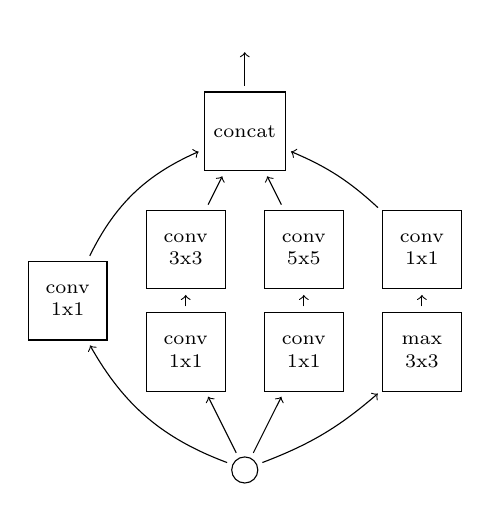
\begin{tikzpicture}[
box/.style={
	draw,
	minimum width=1cm,
	minimum height=1cm,
	font=\scriptsize,
	align=center
}, pil/.style={
	->,
	shorten <=2pt,
	shorten >=2pt
}]

\node[] (out) at (0,2.7) {};

\node[box] (concat) at (0,1.5) {concat};

\node[box] (bll) at (-2.25,-0.65) {conv \\ 1x1};

\node[box] (tl) at (-.75,0) {conv \\ 3x3};
\node[box] (tr) at (.75,0) {conv \\ 5x5};
\node[box] (trr) at (2.25,0) {conv \\ 1x1};

\node[box] (bl) at (-.75,-1.3) {conv \\ 1x1};
\node[box] (br) at (.75,-1.3) {conv \\ 1x1};
\node[box] (brr) at (2.25,-1.3) {max \\ 3x3};

\node[draw,circle] (input) at (0,-2.8) {};

\draw[pil] (concat) edge (out);

\draw[pil, bend left=20] (input) edge (bll);
\draw[pil] (input) edge (bl);
\draw[pil] (input) edge (br);
\draw[pil, bend right=10] (input) edge (brr);

\draw[pil] (bl) edge (tl);
\draw[pil] (br) edge (tr);
\draw[pil] (brr) edge (trr);

\draw[pil, bend left=20] (bll) edge (concat);
\draw[pil] (tl) edge (concat);
\draw[pil] (tr) edge (concat);
\draw[pil, bend right=10] (trr) edge (concat);
\end{tikzpicture}
		}
	\end{tabular}
	\qquad\qquad
	\begin{tabular}{@{}c@{}}
		\subfloat{
			\begin{tikzpicture}[scale=0.8,
box/.style={
	draw,
	minimum width=0.7cm,
	minimum height=0.7cm,
	font=\tiny,
	inner sep = 0pt,
	align=center
}, pil/.style={
	->,
	shorten <=2pt,
	shorten >=2pt
}, add/.style={
	draw,
	circle,
	inner sep = 0.2pt,
	font=\small,
	align=center
}]

\node[draw, diamond, font=\tiny, inner sep=0.5pt, align=center] (out) at (0,4) {$h_{4+1}$};
\node[add] (add) at (0,2.75) {+};
\node[draw, diamond, font=\tiny, inner sep=0.5pt, align=center] (layer2) at (0,1.5) {$h_{3+i}$};
\node[draw, diamond, font=\tiny, inner sep=0.5pt, align=center] (layer1) at (0,0) {$h_{2+i}$};
\node[draw, diamond, font=\tiny, inner sep=0.5pt, align=center] (input) at (0,-1.5) {$h_{1+i}$};

\draw[decorate,decoration={brace,mirror}] (-.7,2) -- (-.7,-.5);
\node[] at (-1.6,.75) {$\mathcal{F}(\bm{x})$};
\node[] at (-1.2,-1.5) {$\bm{x}$};
\node[] at (-1.2,2.75) {$\mathcal{H}(\bm{x})$};

\draw[pil] (input) edge (layer1);
\draw[pil] (layer1) edge (layer2);
\draw[pil] (layer2) edge (add);
\draw[pil] (add) edge (out);

\draw[pil,out=0,in=0] (input) edge (add);

\end{tikzpicture}
		}
	\end{tabular}
	
	\caption[Various advanced DCNN architectures]{Inception block of GoogLeNet~\cite{szegedy2015going} (2014, left) and a skip connection of a residual network~\cite{he2016deep} (2015, right).}
	\label{fig:inception_block}
\end{figure}

By looking at those described networks it seems that adding more layers is beneficial. But increasing the depth of suitably deep models can lead to accuracy degradation~\cite{he2016deep}. Yet this is not caused by overfitting since we can also observe higher training error. It could be partly due to vanishing or exploding gradients even though there are methods to moderate the problem such as clever weight initialization or gradient normalization. To tackle the problem a deep residual learning framework~\cite{he2016deep} was proposed. Instead of training a set of layers to fit a desired underlying mapping $\mathcal{H}(\bm{x})$ directly, it lets layers to fit a residual mapping $\mathcal{F}(\bm{x})-\bm{x}$ such that $\mathcal{H}(\bm{x}) = \mathcal{F}(\bm{x})+\bm{x}$. In neural networks, it can be realized by ``skip connections'' (Figure~\ref{fig:inception_block}). ResNet-152, a DCNN utilizing this idea  with whooping 152 layers, achieved 4.49\% top-5 error rate on ILSVRC in 2015.

The most recent attempts to automate a network's architecture engineering process were made using reinforcement learning (RL)~\cite{zoph2016neural,zoph2017learning}. The methods utilize a controller recurrent neural network (RNN) that predicts a network architecture. This architecture is then trained and its achieved accuracy is used to scale the gradients to update the RNN controller. Despite being extremely computationally demanding needing thousands of GPU-hours even on small datasets, \cite{zoph2017learning} shows that architectures learned on CIFAR-10 can translate easily to ImageNet's ILSVRC achieving best results ever with 3.8\% top-5 error rate. Even smaller networks using the same structure outperform equivalently-sized human-designed models. A cell of the best performing architecture can be seen in Figure~\ref{fig:nasnet_block}.

\begin{figure}
	\centering
	\begin{tikzpicture}[scale=0.8,
box/.style={
	draw,
	minimum width=0.7cm,
	minimum height=0.7cm,
	font=\tiny,
	inner sep = 0pt,
	align=center
}, pil/.style={
	->,
	shorten <=2pt,
	shorten >=2pt
}, add/.style={
	draw,
	circle,
	inner sep = 0.2pt,
	font=\small,
	align=center
}]


\node[draw, diamond, font=\tiny, inner sep=0.5pt, align=center] (out) at (0,3.9) {$h_{i+1}$};

\node[box, inner sep=2pt] (concat) at (0,2.5) {concat};

\draw[pil] (concat) edge (out);

\node[add] (rr) at (4.2,1.1) {+};
\node[add] (r) at (2.1,1.1) {+};
\node[add] (c) at (0,1.1) {+};
\node[add] (l) at (-2.1,1.1) {+};
\node[add] (ll) at (-4.2,1.1) {+};

\draw[pil] (rr) edge (concat);
\draw[pil] (r) edge (concat);
\draw[pil] (c) edge (concat);
\draw[pil] (l) edge (concat);
\draw[pil] (ll) edge (concat);


\node[box] (rr1) at (4.68,0) {sep \\ 3x3};
\node[box] (rr2) at (3.72,0) {sep \\ 5x5};

\node[box] (r1) at (2.58,0) {avg \\ 3x3};
\node[box] (r2) at (1.62,0) {avg \\ 3x3};

\node[box] (c1) at (.48,0) {iden \\ tity};
\node[box] (c2) at (-.48,0) {avg \\ 3x3};

\node[box] (l1) at (-1.62,0) {sep \\ 5x5};
\node[box] (l2) at (-2.58,0) {sep \\ 3x3};

\node[box] (ll1) at (-3.72,0) {iden \\ tity};
\node[box] (ll2) at (-4.68,0) {sep \\ 3x3};

\draw[pil,out=90,in=315] (rr1) edge (rr);
\draw[pil,out=90,in=225] (rr2) edge (rr);

\draw[pil,out=90,in=315] (r1) edge (r);
\draw[pil,out=90,in=225] (r2) edge (r);

\draw[pil,out=90,in=315] (c1) edge (c);
\draw[pil,out=90,in=225] (c2) edge (c);

\draw[pil,out=90,in=315] (l1) edge (l);
\draw[pil,out=90,in=225] (l2) edge (l);

\draw[pil,out=90,in=315] (ll1) edge (ll);
\draw[pil,out=90,in=225] (ll2) edge (ll);


\node[draw, diamond, font=\tiny, inner sep=0.5pt, align=center] (h1) at (0,-1.4) {$h_{i-1}$};
\node[text height=0.333cm, execute at begin node=\color{black}$\vdots$] (hidden) at (0,-2.3) {};
\node[draw, diamond, font=\tiny, inner sep=0.5pt, align=center] (h2) at (0,-3.2) {$h_{i-2}$};

\draw[pil,out=135,in=270] (h1) edge (c2);
\draw[pil,out=180,in=270] (h1) edge (l1);
\draw[pil,out=180,in=270] (h1) edge (ll1);
\draw[pil,out=180,in=270] (h1) edge (ll2);


\draw[pil,out=30,in=270,dashed] (h2) edge (c1);
\draw[pil,out=180,in=270,dashed] (h2) edge (l2);
\draw[pil,out=0,in=270,dashed] (h2) edge (r1);
\draw[pil,out=0,in=270,dashed] (h2) edge (r2);
\draw[pil,out=0,in=270,dashed] (h2) edge (rr1);
\draw[pil,out=0,in=270,dashed] (h2) edge (rr2);
\end{tikzpicture}
	
	\caption[A state-of-the-art block of NASNet-A]{A state-of-the-art block of NASNet-A~\cite{zoph2017learning} (2017), created by a recurrent neural network, outperformed all blocks ever designed by humans.}
	\label{fig:nasnet_block}
\end{figure}

\section{Other Approaches to Annotation}

It is not uncommon an image given for annotation contains dozens of objects, then the classical approach to image classification starts to fall apart since a standard softmax classification layer prefers to assign only one class. Ordinarily, multiple cutouts of an image are taken and annotated separately, the final classification is a mean of distributions for each cutout. It may be sufficient for the task but it does not give us locations of the objects. To obtain a bounding box of an object in an image, a region-based convolutional network (R-CNN) has been proposed~\cite{ren2015faster}. It utilizes two deep convolutional networks, a region proposal network (RPN) suggesting regions of interest and a standard classification DCNN annotating suggested regions. RPN uses first convolutional layers of a standard DCNN such as \cite{simonyan2014very} to generate a feature map. Then a small network $\mathcal{N}$ takes an $n\times n$ spatial window of the feature map and predicts $k$ bounding boxes, for each box also stating a probability it contains an object (Figure \ref{fig:faster_RCNN}). Depending on the size of the feature map and number $k$, which is usually set to $9$, the network generates thousands of regions of interest. The most probable ones are then taken.


\begin{figure}
	\centering
	\begin{tikzpicture}[scale=.8]

	% Define the macro.
	% 1st argument: Height and width of the layer rectangle slice.
	% 2nd argument: Depth of the layer slice
	% 3rd argument: X Offset --> use it to offset layers from previously drawn layers.
	% 4th argument: Options for filldraw.
	% 5th argument: Y Offset --> Use it when an output needs to be fed to multiple layers that are on the same X offset.


	\newcommand{\networkLayer}[6]{
		\def\a{#1} % Used to distinguish input resolution for current layer.
		\def\c{#2} % Width of the cube to distinguish number of input channels for current layer.
		\def\t{#3} % X offset for current layer.
		\ifthenelse {\equal{#5} {}} {\def\y{0}} {\def\y{#5}} % Y offset for current layer.

		% Recolor visible surfaces
		\ifthenelse {\equal{#4} {}} {
			\draw[line width=0.1mm](\t,\a+\y,0+\y) -- (\t,0+\y,0+\y) -- (\t+\c,0+\y,0+\y);
			\draw[line width=0.1mm](\t,0+\y,0+\y) -- (\t,0+\y,\a+\y);
		} {
			\filldraw[#4] (\t,0,\a) -- (\c+\t,0,\a) -- (\c+\t,\a,\a) -- (\t,\a,\a) -- (\t,0,\a);
			\filldraw[#4] (\t,\a,\a) -- (\c+\t,\a,\a) -- (\c+\t,\a,0) -- (\t,\a,0);
			\filldraw[#4] (\c+\t,0,\a) -- (\c+\t,0,0) -- (\c+\t,\a,0) -- (\c+\t,\a,\a);
		}

		% Draw the layer body.
		\draw[line width=0.1mm](\c+\t,0+\y,0+\y) -- (\c+\t,\a+\y,0+\y) -- (\t,\a+\y,0+\y); % back plane
		\draw[line width=0.1mm](\t,0+\y,\a+\y) -- (\c+\t,0+\y,\a+\y) -- (\c+\t,\a+\y,\a+\y) -- (\t,\a+\y,\a+\y) -- (\t,0+\y,\a+\y); % front plane

		\draw[line width=0.1mm](\c+\t,0+\y,0+\y) -- (\c+\t,0+\y,\a+\y);
		\draw[line width=0.1mm](\c+\t,\a+\y,0+\y) -- (\c+\t,\a+\y,\a+\y);
		
		\ifthenelse {\equal{#6} {}} {
			\draw[line width=0.1mm](\t,\a+\y,0+\y) -- (\t,\a+\y,\a+\y);
		} {
			\draw[line width=0.1mm](\t,\a+\y,0+\y) -- (\t,\a+\y,\a+\y) node[midway, anchor=center,sloped, above=-2.5pt, font=\scriptsize] {#6};
		}
	}


	% ENCODER
	\networkLayer{4.0}{0.1}{0.0}{color=white}{}{}
	\networkLayer{3.7}{0.1}{0.2}{color=white}{}{}
	\networkLayer{3.4}{0.1}{0.4}{color=white}{}{}
	\node[text height=0.333cm, execute at begin node=\color{black}$\dots$, scale=1] at (1.25,2,2) {};
	\networkLayer{3.0}{0.3}{2}{}{}{}
	\networkLayer{1}{0.3}{2}{}{1}{$n$}
	
	\networkLayer{.3}{3}{3.4}{}{1}{}
	
	\draw[line width=0.1mm,dashed](2.3,2,1) -- (3.4,1.3,1) {};
	\draw[line width=0.1mm,dashed](2.3,2,2) -- (3.4,1.3,1.3) {};
	\draw[line width=0.1mm,dashed](2.3,1,1) -- (3.4,1,1) {};
	\draw[line width=0.1mm,dashed](2.3,1,2) -- (3.4,1,1.3) {};
	
	
	\draw[line width=0.1mm](8,1,1) -- (8,1,-2) -- (8.3,1,-2) -- (8.3,1,1) node[midway, anchor=center, sloped, below, font=\tiny] {$k$ boxes} -- (8,1,1);
	
	\draw[line width=0.1mm](8,1,1.3) -- (8,1,4.3) -- (8.3,1,4.3) -- (8.3,1,1.3) node[midway, anchor=center, sloped, below, font=\tiny] {$k$ probabilities} -- (8,1,1.3);
	
	\draw[line width=0.1mm,dashed](8,1,1) -- (6.4,1,1.15) {};
	\draw[line width=0.1mm,dashed](8,1,-2) -- (6.4,1,1) {};

	\draw[line width=0.1mm,dashed](8,1,4.3) -- (6.4,1,1.3) {};
	\draw[line width=0.1mm,dashed](8,1,1.3) -- (6.4,1,1.15) {};
	
	\draw[decorate,decoration={brace,mirror}] (0.0,0,4.3) -- (2.6,0,4.3) node[midway, anchor=center,sloped, below=0.1, font=\scriptsize] {CNN};
	
	\draw[decorate,decoration={brace,mirror}] (2.8,0,4.3) -- (8,0,4.3) node[midway, anchor=center,sloped, below=0.1, font=\scriptsize] {Fully-Connected Network $\mathcal{N}$};

\end{tikzpicture}
	
	\caption[A region-based convolutional network]{A region-based convolutional network~\cite{ren2015faster} (2016), generating $k$ bounding boxes for each sliding window $n\times n$.}
	\label{fig:faster_RCNN}
\end{figure}

Shown in~\cite{zeiler2014visualizing}, first layers of CNN learn low features such as lines and corners with later layers learning more complex representations of images. This can be used for semi-supervised learning. Deep convolutional representations learned on similar annotated dataset are applied to new tasks where supervised learning is expensive to do~\cite{donahue2014decaf}. $K$-nearest neighbors algorithm can be then used to annotate unknown images by projecting them onto a feature space of the network's later layers. Such an approach can be scaled to much bigger datasets than ImageNet, working reasonably well even on YFCC100M~\cite{amato2017searching}.